\chapter{MÔ PHỎNG HOẠT ĐỘNG CỦA ROBOT}
     \section{Thông số của robot}
          \hspace*{0.6cm}Thực hiện mô phỏng chuyển động của Robot sau khi tìm được hàm truyền của động cơ bằng cách nhúng hàm truyền động cơ,
          bộ điều khiển tốc độ, sai số cảm biến cùng với bộ điều khiển vị trí bám line với các thông số như sau:
          \begin{table}[h]
               \centering
               \begin{tabular}{|l|c|}
               \hline
               \multicolumn{2}{|c|}{\textbf{Thông số hình học}} \\
               \hline
               Bán kính bánh xe, $r$ & 68 mm \\
               \hline
               Khoảng cách từ tâm dây cảm biến đến trục bánh dẫn động, $a$ & 72 mm \\
               \hline
               Khoảng cách dọc trục giữa tâm 2 bánh xe, $b$ & 220 mm \\
               \hline
               \multicolumn{2}{|c|}{\textbf{Thời gian}} \\
               \hline
               Thời gian lấy mẫu bộ điều khiển động cơ, $t_{\text{s}}$ & 0.01 s \\
               \hline
               Thời gian lấy mẫu bộ điều khiển bám line, $t_{\text{đk}}$ & 0.05 s \\
               \hline
               \multicolumn{2}{|c|}{\textbf{Bộ điều khiển PID}} \\
               \hline
               Vị trí bám line & $K_P = 0.078$; $K_D = 0.015$ \\
               \hline
               Động cơ phải & $K_P = 1.0852$; $K_I = 13.6563$ \\
               \hline
               Động cơ trái & $K_P = 1.0673$; $K_I = 13.948$ \\
               \hline
               \multicolumn{2}{|c|}{\textbf{Thông số động học}} \\
               \hline
               Vận tốc của robot, $v$ & 500 mm/s \\
               \hline
               Vận tốc của robot lúc vào cua, $v_{\text{r}}$ & 300 mm/s \\
               \hline
               Góc lệch ban đầu, $p$ & $\pi$ \\
               \hline
               \end{tabular}
               \label{tab:robot_specifications}
               \caption{Thông số đầu vào mô phỏng chuyển động của robot}
          \end{table}
     \section{Thực hiện mô phỏng}
     \hspace*{0.6cm}Mô phỏng bằng phần mềm MATLAB, bước đầu tiên là tạo sa bàn với các kích thước như trong đầu bài
     \begin{figure}[H]
          \centering
          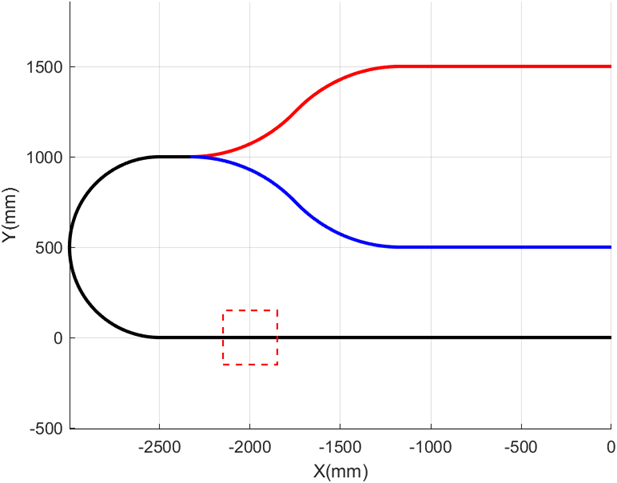
\includegraphics[width=0.8\textwidth]{pictures/chapter8/saban.png}
          \caption{Hình ảnh sa bàn}
          \label{saban}
     \end{figure}
     \hspace*{0.6cm}Trong đó đường line màu đỏ và màu xanh lần lượt thể hiện nhánh rẽ khi xe nhận được khối hàng màu đỏ và xanh. Tại 
     


     \section{Kết quả mô phỏng}
     \newpage
          \subsection{Khối hàng đỏ}
               \begin{figure}[H]
                    \centering
                    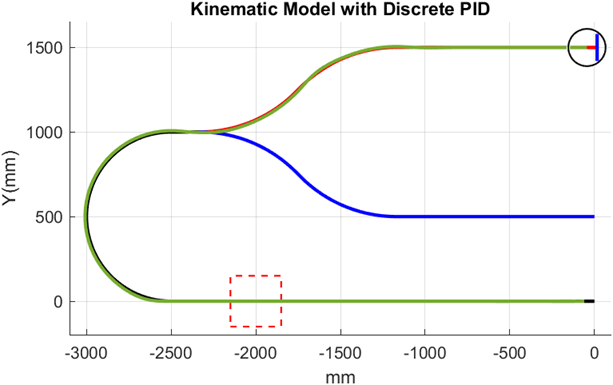
\includegraphics[width=1\textwidth]{pictures/chapter8/trajec_red.png}
                    \caption{Quỹ đạo đi khi nhận khối hàng đỏ}
                    \label{tra_red}
               \end{figure}
               \begin{figure}[H]
                    \centering
                    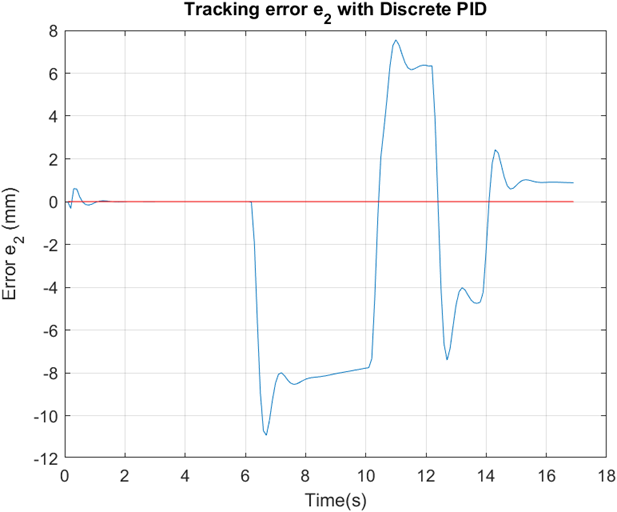
\includegraphics[width=0.8\textwidth]{pictures/chapter8/err_red.png}
                    \caption{Lỗi quỹ đạo e2 khi nhận khối hàng đỏ}
                    \label{err_red}
               \end{figure}
          \subsection{Khối hàng xanh}
               \begin{figure}[H]
                    \centering
                    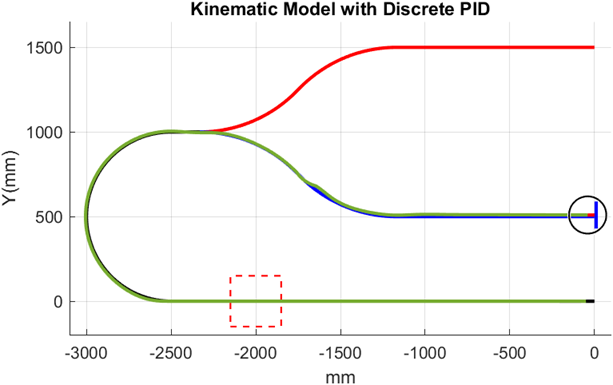
\includegraphics[width=0.8\textwidth]{pictures/chapter8/trajec_blue.png}
                    \caption{Quỹ đạo đi khi nhận khối hàng xanh}
                    \label{tra_blue}
               \end{figure}
               \begin{figure}[H]
                    \centering
                    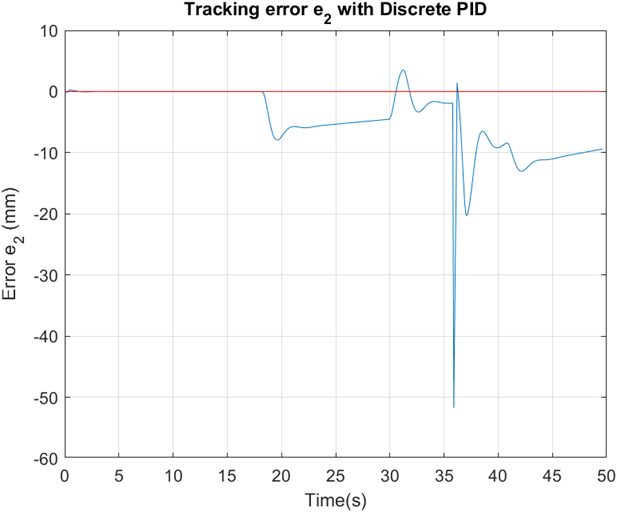
\includegraphics[width=0.8\textwidth]{pictures/chapter8/err_blue.png}
                    \caption{Lỗi quỹ đạo e2 khi nhận khối hàng xanh}
                    \label{err_blue}
               \end{figure}